% ******************************************************** %
%              TEMPLATE DE INFORME ORGA2 v0.1              %
% ******************************************************** %
% ******************************************************** %
%                                                          %
% ALGUNOS PAQUETES REQUERIDOS (EN UBUNTU):                 %
% ========================================
%                                                          %
% texlive-latex-base                                       %
% texlive-latex-recommended                                %
% texlive-fonts-recommended                                %
% texlive-latex-extra?                                     %
% texlive-lang-spanish (en ubuntu 13.10)                   %
% ******************************************************** %


\documentclass[a4paper]{article}
\usepackage[spanish]{babel}
\usepackage[utf8]{inputenc}
\usepackage{charter}   % tipografia
\usepackage{graphicx}
%\usepackage{makeidx}
\usepackage{paralist} %itemize inline

%\usepackage{float}
%\usepackage{amsmath, amsthm, amssymb}
%\usepackage{amsfonts}
%\usepackage{sectsty}
%\usepackage{charter}
%\usepackage{wrapfig}
%\usepackage{listings}
%\lstset{language=C}

% \setcounter{secnumdepth}{2}
\usepackage{underscore}
\usepackage{caratula}
\usepackage{url}
\usepackage{array}
\usepackage{lineno}


% ********************************************************* %
% ~~~~~~~~              Code snippets             ~~~~~~~~~ %
% ********************************************************* %

\usepackage{color} % para snipets de codigo coloreados
\usepackage{fancybox}  % para el sbox de los snipets de codigo

\definecolor{litegrey}{gray}{0.94}

\newenvironment{codesnippet}{%
	\begin{Sbox}\begin{minipage}{\textwidth}\sffamily\small}%
	{\end{minipage}\end{Sbox}%
		\begin{center}%
		\vspace{-0.4cm}\colorbox{litegrey}{\TheSbox}\end{center}\vspace{0.3cm}}



% ********************************************************* %
% ~~~~~~~~         Formato de las páginas         ~~~~~~~~~ %
% ********************************************************* %

\usepackage{fancyhdr}
\pagestyle{fancy}

%\renewcommand{\chaptermark}[1]{\markboth{#1}{}}
\renewcommand{\sectionmark}[1]{\markright{\thesection\ - #1}}

\fancyhf{}

\fancyhead[LO]{Sección \rightmark} % \thesection\ 
\fancyfoot[LO]{\small{Daniel Nuñez, Nicolás Fantagossi, Alejo Salvador}}
\fancyfoot[RO]{\thepage}
\renewcommand{\headrulewidth}{0.5pt}
\renewcommand{\footrulewidth}{0.5pt}
\setlength{\hoffset}{-0.8in}
\setlength{\textwidth}{16cm}
%\setlength{\hoffset}{-1.1cm}
%\setlength{\textwidth}{16cm}
\setlength{\headsep}{0.5cm}
\setlength{\textheight}{25cm}
\setlength{\voffset}{-0.7in}
\setlength{\headwidth}{\textwidth}
\setlength{\headheight}{13.1pt}

\renewcommand{\baselinestretch}{1.1}  % line spacing

% ******************************************************** %


\begin{document}


\thispagestyle{empty}
\materia{Organización del Computador II}
\submateria{Segundo Cuatrimestre de 2014}
\titulo{Trabajo Práctico II}
\subtitulo{Procesamiento SIMD}
\integrante{Fantagossi Nicolas Ezequiel}{229/14}{nicolasfantagossi@gmail.com}
\integrante{Nuñez Morales Carlos Daniel}{732/08}{cdani.nm@gmail.com}

\maketitle
\newpage

\thispagestyle{empty}
\vfill
\begin{abstract}
En el presente trabajo se analiza la diferencia en performance que pueden provocar los misses en la cache y un analisis de performance vs. calidad al utilizar menor presicion al calcular datos.
\end{abstract}

\thispagestyle{empty}
\vspace{3cm}
\tableofcontents
\newpage


%\normalsize
\newpage

\section{Objetivos generales}

El objetivo de este Trabajo Práctico es analizar la importancia que puede tener la cache en la performance de un programa. Por otro lado, analizamos las ventajas y consecuencias de utilizar menor precision en calculos, comparando la performance ganada vs. la calidad perdida.

\section{Contexto}

\subsection{Smalltiles}
El filtro consiste en generar cuatro miniaturas de una imagen fuente en una misma imagen final. Cada miniatura posee la mitad de dimensiones.

\begin{center}
 \begin{tabular}{m{4cm} m{2cm} m{4cm}}
   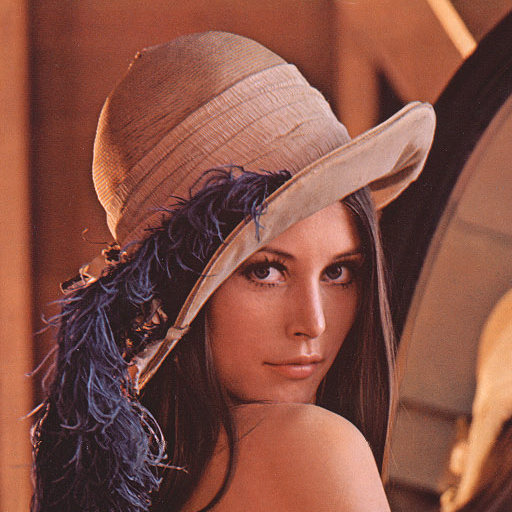
\includegraphics[width=0.2\textwidth]{imagenes/lena.png} &
    \begin{tabular}{c}
      $\longrightarrow$
    \end{tabular} &
   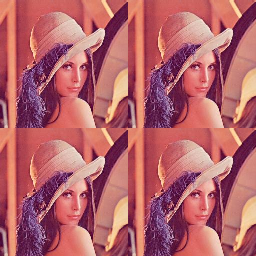
\includegraphics[width=0.2\textwidth]{imagenes/lena-smalltiles.png} \\
 \end{tabular}
\end{center}

\subsection{Rotar}
El filtro consiste en intercambiar los valores de los canales entre si. En el resultado final, los canales quedan ordenados de la siguiente manera:

\begin{center}
 \begin{tabular}{m{4cm} m{4cm} m{4cm}}
    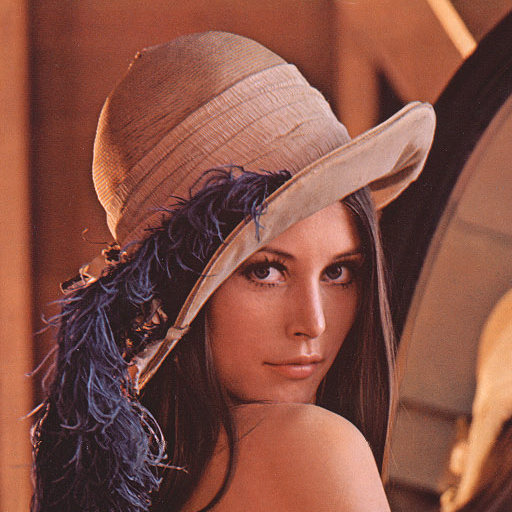
\includegraphics[width=0.2\textwidth]{imagenes/lena.png} &
    \begin{tabular}{ccc}
       R & $\longrightarrow$ & G \\
       G & $\longrightarrow$ & B \\
       B & $\longrightarrow$ & R \\
       Alpha & $\longrightarrow$ & Alpha
    \end{tabular} &
    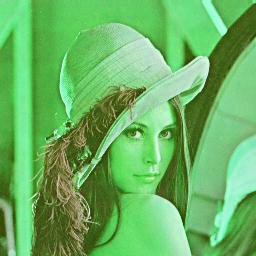
\includegraphics[width=0.2\textwidth]{imagenes/lena-rotar-canales.png} \\
 \end{tabular}
\end{center}

\subsection{Pixelar}
El filtro consiste en tomar cuadrados de 2x2 pixeles de una imagen base, calcular el promedio entre ellos y copiar el pixel obtenido a los 4 pixeles correspondientes de la imagen destino.

\begin{center}
 \begin{tabular}{m{4cm} m{2cm} m{4cm}}
    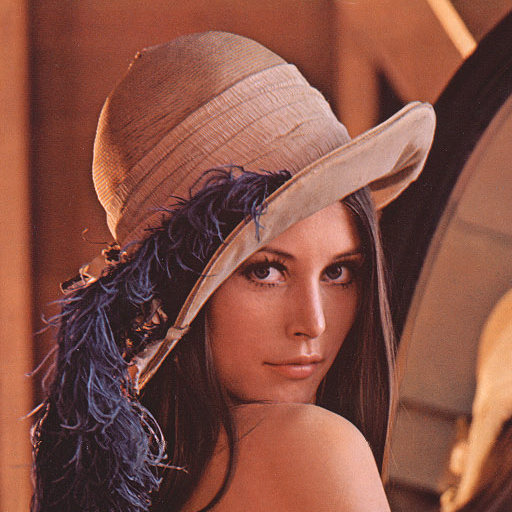
\includegraphics[width=0.2\textwidth]{imagenes/lena.png} &
    \begin{tabular}{c}
      $\longrightarrow$
    \end{tabular} &
    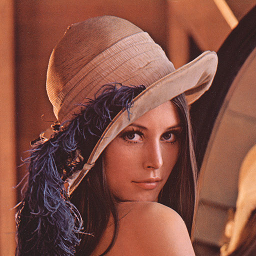
\includegraphics[width=0.2\textwidth]{imagenes/lena-pixelar.png} \\
 \end{tabular}
\end{center}

\subsection{Combinar}
El filtro consiste en tomar dos imagenes, A y B, y combinarlas segun un parametro alpha (entre 0 y 255) que indica cuanto de la imagen B se aplicará. Un valor máximo de 255 no modifica la imagen A, mientras que un valor de 0 dejará unicamente la imagen B.

\begin{center}
 \begin{tabular}{m{4cm} m{2cm} m{4cm}}
    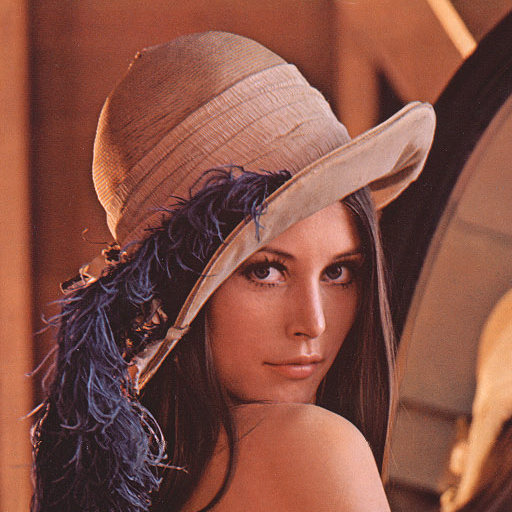
\includegraphics[width=0.2\textwidth]{imagenes/lena.png} &
    \begin{tabular}{c}
      $\longrightarrow$
    \end{tabular} &
    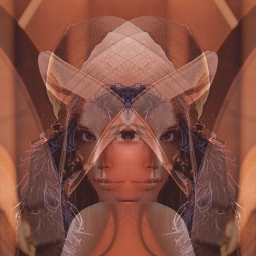
\includegraphics[width=0.2\textwidth]{imagenes/lena-combinar.png} \\
 \end{tabular}
\end{center}

\subsection{Colorizar}
El filtro consiste en analizar cada pixel y sus vecinos obteniendo el maximo para cada canal entre todos ellos. Luego, para cada canal, se analiza de acuerdo a las siguientes reglas:

\begin{center}
\begin{displaymath}
 \phi_R(i, j) = \left\{
\begin{array}{l l}
  		(1 + \alpha) & si\ max_R(i,j) \geq max_G(i,j) y max_R(i,j) \geq max_B(i,j) \\
  		(1 - \alpha) & si\ no
\end{array}
\right.
\end{displaymath}

\begin{displaymath}
 \phi_G(i, j) = \left\{
\begin{array}{l l}
  		(1 + \alpha) & si\ max_R(i,j) < max_G(i,j) y max_G(i,j) \geq max_B(i,j)\\
  		(1 - \alpha) & si\ no
\end{array}
\right.
\end{displaymath}

\begin{displaymath}
\phi_B(i, j) = \left\{
\begin{array}{l l}
  		(1 + \alpha) & si\ max_R(i,j) < max_B(i,j) y max_G(i,j) < max_B(i,j)\\
  		(1 - \alpha) & si\ no
\end{array}
\right.
\end{displaymath}
\end{center}

Una vez obtenido cada $\phi_c$, se calcula el mínimo entre $\phi_c * max_c(i,j)$ y 255 y se utiliza este como valor para el canal $c$ del pixel $(i,j)$ destino.

\begin{center}
 \begin{tabular}{m{4cm} m{2cm} m{4cm}}
    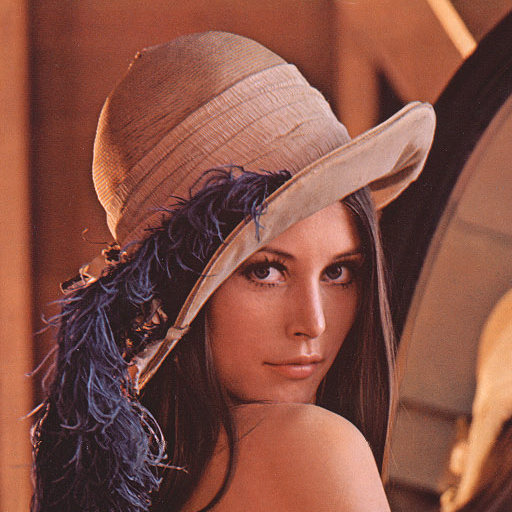
\includegraphics[width=0.2\textwidth]{imagenes/lena.png} &
    \begin{tabular}{c}
      $\longrightarrow$
    \end{tabular} &
    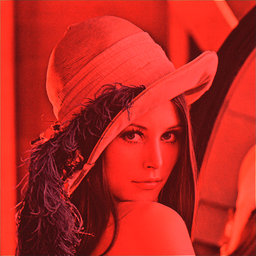
\includegraphics[width=0.2\textwidth]{imagenes/lena-colorizar.png} \\
 \end{tabular}
\end{center}
\clearpage
\section{Implementacion}


\subsection{Smalltiles}
Para aplicar el filtro, se recorre la matriz de a filas (ignorando las filas pares, ya que serian las impares de la imágen al estar invertidas y por como esta definido el filtro solo interesan los pixeles en fila y columna par) y de a 4 columnas/pixeles (dado que es el maximo que se puede guardar en un registro xmm). En el ciclo exterior recorremos cada fila impar, mientras que en el interior procesamos las columnas. Como podría suceder que la cantidad de columnas de la imagen sea de la forma 4K+2 con K entero y el algoritmo recorre de a 4 por fila, debe hacerse un caso especial en el cual de pasar eso se recorren los ultimos 2 elementos de forma independiente, lo cuál no se hara con SIMD ya que no se ganaría nada al solo tener que usar el segundo elemento de los 2 al momento de escribir en los lugares correspondientes.

El algoritmo de procesamiento es el siguiente:

\begin{itemize}
    \itemsep0em
    \item[-]
        Buscamos en memoria 4 pixeles, px1, px2, px3,  y px4. figura~\ref{nombrepixeles2}
        \begin{figure}[!htb]
          \begin{center}
        	\includegraphics[scale=0.2]{imagenes/diagramas/smalltiles/nombrepixeles2.png}
        	\caption{Etiquetas de pixels}
        	\label{nombrepixeles2}
          \end{center}
        \end{figure}

    \item[-]
        Ahora haremos un shuffle para conseguir que los elementos px2 y px4 queden en la low-word. figura~\ref{shufflePixeles2}
        \begin{figure}[!htb]
          \begin{center}
        	\includegraphics[scale=0.2]{imagenes/diagramas/smalltiles/shuffle2.png}
        	\caption{Shuffle}
        	\label{shufflePixeles2}
          \end{center}
        \end{figure}
    \item[-]
        Ahora guardo los 2 elementos de la low-word en las 4 posiciones que corresponde en la imagen de destino. figura~\ref{output}
        \begin{figure}[!htb]
          \begin{center}
        	\includegraphics[scale=0.3]{imagenes/diagramas/smalltiles/output.png}
        	\caption{Guardar}
        	\label{output}
          \end{center}
        \end{figure}

\end{itemize}

\clearpage
\subsubsection*{Codigo fuente:}
\begin{codesnippet}
\begin{internallinenumbers}
\begin{verbatim}
.ciclo_columna:
		cmp rdx, 0
		je .fin
		mov rdi, r10
		mov rsi, r11
		mov rbx, r12
		mov rcx, r13
		sar rcx, 1		; proceso dos pixels por vez
		.ciclo_fila:
			movdqu xmm0, [rdi]
			pshufd xmm1, xmm0, 0x08
			movq [rsi], xmm1
			movq [rsi+r13*4], xmm1
			movq [rbx], xmm1
			movq [rbx+r13*4], xmm1
			add rdi, 16
			add rsi, 8
			add rbx, 8
			
			loop .ciclo_fila
			
		mov rcx, r13
		shr rcx, 1
		shl rcx, 1
		sub rcx, r13
		cmp rcx, 0
		je .salir_c_fila
		mov eax, [rdi]
		mov [rsi], eax
		mov [rsi+r13*4], eax
		mov [rbx], eax
		mov [rbx+r13*4], eax
				
		.salir_c_fila:
				lea r10, [r10+r8*2]
				lea r11, [r11+r9]
				lea r12, [r12+r9]
				dec rdx
				jmp .ciclo_columna
\end{verbatim}
\end{internallinenumbers}
\end{codesnippet}

\clearpage
\subsection{Rotar}

Para aplicar el filtro, se recorre la imagen de una fila y de a 4 columnas/pixeles (dado que es el maximo que se puede guardar en un registro xmm). En el ciclo exterior recorremos las filas, mientras que en el interior procesamos las columnas. En caso de que las filas tengan una cantidad de pixles que no sea multiplo de 4 se seguira haciendo exactamente el mismo shufle, pero solamente se copiaran la cantidad de elementos que corresponda en el último paso. El proceso de determinar la congruencia modulo 4 se hace simplemente usando un compare.

El algoritmo de procesamiento para cada iteración en la fila es el siguiente:

\begin{itemize}
    \itemsep0em
    \item[-]
        Buscamos en memoria 4 pixeles, px1, px2, px3, px4 figura~\ref{leer}
        \begin{figure}[!htb]
          \begin{center}
        	\includegraphics[scale=0.4]{imagenes/diagramas/rotar/leer.png}
        	\caption{Etiquetas de pixels}
        	\label{leer}
          \end{center}
        \end{figure}
    \item[-]
        Hacemos un shufle de forma tal que se roten los colores de cada uno de dichos pixeles.
         figura~\ref{shufflerotar}
        \begin{figure}[!htb]
          \begin{center}
        	\includegraphics[scale=0.4]{imagenes/diagramas/rotar/shufflerotar.png}
        	\caption{Shuffle}
        	\label{shufflerotar}
          \end{center}
        \end{figure}
    \item[-]
        Guardamos en el resutlado lo obtenido con el shuffle.
   \end{itemize}
   

\subsubsection*{Codigo fuente:}
\begin{codesnippet}
\begin{internallinenumbers}
\begin{verbatim}
cicloFilas:	  
  	 cmp rax, 0		;comparo el alto con 0 a ver si termine de procesar todas las filas	
	   je finRotar
	   mov rdi, r10
	   mov rsi, r11
	   mov rcx, rdx
	   shr rcx, 2		;proceso de a 4 pixeles

		cicloColumnas:

			   movdqu xmm0, [rdi]	;xmm0= |a15|....|a0|	;uso xmm0 para rojo
			   pshufb xmm0,xmm1
			   movdqu [rsi], xmm0		;muevo a memoria	

			   add rdi, 16
			   add rsi, 16			
			   loop	cicloColumnas

		;sino es multiplo de 4 ntonces me faltan procesar 3, 2 o 1 pixel
			mov rcx, rax
			shr rcx, 2
			shl rcx, 2
			sub rcx, rax		;esta resta puede ser: 0, -1, -2 o -3
			cmp rcx, 0
			je .no_faltan
			cmp rcx, -1
			je .faltan_1
			cmp rcx, -2
			je .faltan_2
			;si no salta entonces faltaba 3 pixeles:
			
			movdqu xmm0, [rdi]	;xmm0= |a15|....|a0|	;uso xmm0 para rojo
			pshufb xmm0,xmm1
			movq [rsi], xmm0		;muevo a memoria 2 pixeles
			add rsi, 8
			psrldq xmm0, 8
			movd [rsi], xmm0
			jmp .no_faltan
			
			.faltan_1:
			movd xmm0, [rdi]	;xmm0= |a15|....|a0|	;uso xmm0 para rojo
			pshufb xmm0,xmm1
			movd [rsi], xmm0		;muevo 1 pixel memoria	
			jmp .no_faltan
			
			.faltan_2:
			movq xmm0, [rdi]	;xmm0= |a15|....|a0|	;uso xmm0 para rojo
			pshufb xmm0,xmm1
			movq [rsi], xmm0		;muevo a memoria
			jmp .no_faltan	
			

	.no_faltan:

	   add r10, r8			;a rdi le sumo el ancho para apuntar a la proxima fila
	   add r11, r9
	   dec rax			;decremento el contador de filas
	   jmp cicloFilas
\end{verbatim}
\end{internallinenumbers}
\end{codesnippet}
\clearpage

\subsection{Pixelar}

Para aplicar el filtro, se recorre la imagen de a dos filas (ya que para ello se necesitas dos pixeles de la primera, y sus inmediatos superiores de la segunda) y de a 4 columnas/pixeles (dado que es el maximo que se puede guardar en un registro xmm). En el ciclo exterior recorremos cada par de filas, mientras que en el interior procesamos las columnas.

El algoritmo de procesamiento es el siguiente:

\begin{itemize}
    \itemsep0em
    \item[-]
        Buscamos en memoria 4 pixeles por cada linea, px11, px12, px21, px22 y px13, px14, px23, px24. figura~\ref{nombrePixeles}
        \begin{figure}[!htb]
          \begin{center}
        	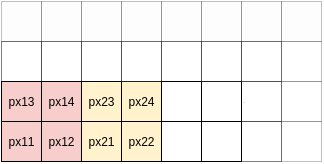
\includegraphics[scale=0.75]{imagenes/diagramas/pixelar/nombrePixeles.png}
        	\caption{Etiquetas de pixels}
        	\label{nombrePixeles}
          \end{center}
        \end{figure}
    \item[-]
        Desempaquetamos extendiendo cada canal, de byte a word, con ceros para obtener 4 registros xmm con cada par de pixeles.
    \item[-]
        Utilizamos SIMD para sumar cada componente de los pixels entre si.
    \item[-]
        Copiamos cada suma parcial a otro registro y hacemos un shuffle para cruzar los datos. figura~\ref{shufflePixeles}
        \begin{figure}[!htb]
          \begin{center}
        	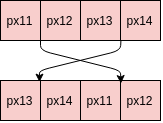
\includegraphics[scale=0.75]{imagenes/diagramas/pixelar/shufflePixeles.png}
        	\caption{Shuffle}
        	\label{shufflePixeles}
          \end{center}
        \end{figure}
    \item[-]
        Utilizando SIMD nuevamente sumamos estas sumas parciales y obtenemos dos registros con las sumas totales de cada grupo de pixeles.
    \item[-]
        Hacemos un shift para dividir por cuatro las sumas y asi obtener el promedio entre los pixeles.
    \item[-]
        Una vez obtenidos los promedios, desempaquetamos todo en un solo registro xmm, el cual contendra los pixeles finales a copiar. figura~\ref{unpackPixeles}
        \begin{figure}[!htb]
          \begin{center}
        	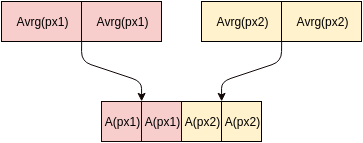
\includegraphics[scale=0.75]{imagenes/diagramas/pixelar/unpackPixeles.png}
        	\caption{Unpack}
        	\label{unpackPixeles}
          \end{center}
        \end{figure}
        \newpage
    \item[-]
        Una vez listo, copiamos los nuevos valores a la imagen destino. figura~\ref{destPixeles}
        \begin{figure}[!htb]
          \begin{center}
        	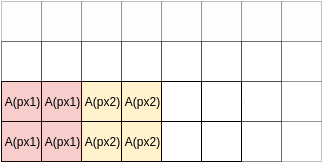
\includegraphics[scale=0.75]{imagenes/diagramas/pixelar/destPixeles.png}
        	\caption{Destino}
        	\label{destPixeles}
          \end{center}
        \end{figure}
\end{itemize}

\subsubsection*{Codigo fuente:}
\begin{codesnippet}
\begin{internallinenumbers}
\begin{verbatim}
movdqu xmm7, [rdi] ; |px11|px12|px21|px22|

movdqu xmm1, xmm7
punpcklbw xmm1, xmm6 ; |px11|px12|
movdqu xmm2, xmm7
punpckhbw xmm2, xmm6 ; |px21|px22|

movdqu xmm7, [rdi + rdx * 4] ; |px13|px14|px23|px24|

movdqu xmm3, xmm7
punpcklbw xmm3, xmm6 ; |px13|px14|
movdqu xmm4 , xmm7
punpckhbw xmm4, xmm6 ; |px23|px24|

paddw xmm1, xmm3 ; |px11 + px13|px12 + px14|
paddw xmm2, xmm4 ; |px21 + px23|px22 + px24|

movdqu xmm3, xmm1
shufpd xmm3, xmm1, 00000001b ; |px12 + px14|px11 + px13|

movdqu xmm4, xmm2
shufpd xmm4, xmm2, 00000001b ; |px22 + px24|px21 + px23|

paddd xmm1, xmm3 ; |px11 + px12 + px13 + px14|px11 + px12 + px13 + px14|
paddd xmm2, xmm4 ; |px21 + px22 + px23 + px24|px21 + px22 + px23 + px24|

psrlw xmm1, 2 ; |avrg(px1)|avrg(px1)|
psrlw xmm2, 2 ; |avrg(px2)|avrg(px2)|

packuswb xmm1, xmm2 ; |avrg(px1)|avrg(px1)|avrg(px2)|avrg(px2)|

movdqu [rsi], xmm1
movdqu [rsi + rdx * 4], xmm1

add rdi, 16
add rsi, 16
\end{verbatim}
\end{internallinenumbers}
\end{codesnippet}
\clearpage
\subsection{Combinar}

La implementacion del filtro consiste en dos partes. En la primera, se procede a invertir la imagen. Para ello se recorre la fuente y, utilizando una mascara, se invierte el orden de los pixeles y se escribe en el destino.
Una vez obtenido el espejo de la fuente en el destino, se procede a aplicar el filtro propiamente dicho.
Dado que en los calculos de este filtro se utilizan floats, y mas allá de que por cada ciclo procesamos 4 pixels, el proceso simultaneo del filtro es de a un pixel; osea, un float de 4 bytes por cada canal.
Para ahorrar instrucciones, antes de iniciar el ciclo, se calcula la division entre el alpha recibido y 255. Con este resultado, copiamos a un segundo registro y por medio de un shuffle lo replicamos en todo un registro, dejandolo listo para utilizar con operaciones de SIMD.
El algoritmo de procesamiento es el siguiente:

\begin{itemize}
    \itemsep0em
    \item[-]
        Buscamos en memoria 4 pixeles de cada imagen y los almacenamos en 2 registros xmm.
    \item[-]
        Por medio de un desempaquetado, extendemos con ceros obteniendo 4 registros con 2 pixeles cada uno. figura~\ref{extenderPixeles}
        \begin{figure}[!htb]
          \begin{center}
        	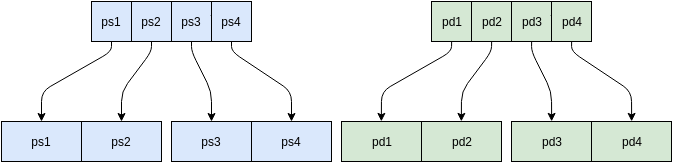
\includegraphics[scale=0.4]{imagenes/diagramas/combinar/extenderPixeles.png}
        	\caption{Detalle de desempaquetado}
        	\label{extenderPixeles}
          \end{center}
        \end{figure}
    \item[-]
        Con los valores desempaquetados, utilizamos SIMD para realizar la resta entre los canales de los pixels.
    \item[-]
        Extendemos nuevamente, esta vez de word a double. Para ello, utilizamos una comparación con cero, del cuál obtenemos una máscara para extender con signo las restas.
    \item[-]
        Realizamos una conversion de cada registro a float.
    \item[-]
        Una vez tenemos los datos en formato de float de presicion simple, realizamos la multiplicacion con el valor precalculado anteriormente.
    \item[-]
        Con los pixeles y procesados, realizamos una nueva conversion para obtener nuevamente enteros.
    \item[-]
        Por medio de dos instrucciones de pack (ambas utilizando saturacion y signo), pasamos los datos de double words a bytes. figura~\ref{empaquetarPixeles}
        \begin{figure}[!htb]
          \begin{center}
        	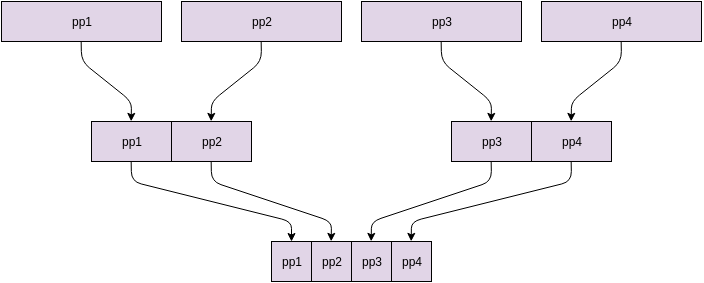
\includegraphics[scale=0.4]{imagenes/diagramas/combinar/empaquetarPixeles.png}
        	\caption{Detalle de empaquetado}
        	\label{empaquetarPixeles}
          \end{center}
        \end{figure}
    \item[-]
        Realizamos una suma entre los datos empaquetados y los pixeles originales obtenidos de la imagen destino.
    \item[-]
        En este punto ya poseemos todos los pixeles con el filtro aplicado, por lo que solo resta escribirlos en la imagen destino y continuar el ciclo.
\end{itemize}

\subsubsection*{Codigo fuente:}
\begin{codesnippet}
\begin{internallinenumbers}
\begin{verbatim}
movdqu xmm1, [rdi] ; xmm1 = |px1s|px2s|px3s|px4s|
movdqu xmm2, [rsi] ; xmm2 = |px1d|px2d|px3d|px4d|
movdqu xmm5, xmm2  ; Lo guardo para utilizar luego.

pxor xmm7, xmm7

movdqu xmm8, xmm1
punpcklbw xmm8, xmm7  ; xmm8  = | px1s | px2s |
movdqu xmm9, xmm1
punpckhbw xmm9, xmm7  ; xmm9  = | px3s | px4s |

movdqu xmm12, xmm2
punpcklbw xmm12, xmm7 ; xmm12 = | px1d | px2d |
movdqu xmm13, xmm2
punpckhbw xmm13, xmm7 ; xmm13 = | px3d | px4d |

psubw xmm8, xmm12     ; xmm8  = | px1s - px1d | px2s - px2d |
psubw xmm9, xmm13     ; xmm9  = | px3s - px3d | px4s - px4d |

movdqu xmm1, xmm8
movdqu xmm2, xmm8
pxor xmm7, xmm7
pcmpgtw xmm7, xmm1
punpcklwd xmm1, xmm7  ; xmm1 = | px1s - px1d |
punpckhwd xmm2, xmm7  ; xmm2 = | px2s - px2d |

movdqu xmm3, xmm9
movdqu xmm4, xmm9
pxor xmm7, xmm7
pcmpgtw xmm7, xmm3
punpcklwd xmm3, xmm7  ; xmm3 = | px3s - px3d |
punpckhwd xmm4, xmm7  ; xmm4 = | px4s - px4d |

cvtdq2ps xmm1, xmm1  ; xmm1 = | f(px1s - px1d) |
cvtdq2ps xmm2, xmm2  ; xmm2 = | f(px2s - px2d) |
cvtdq2ps xmm3, xmm3  ; xmm3 = | f(px3s - px3d) |
cvtdq2ps xmm4, xmm4  ; xmm4 = | f(px4s - px4d) |

mulps xmm1, xmm0  ; xmm1 = | f(px1s - px1d) * d |
mulps xmm2, xmm0  ; xmm2 = | f(px2s - px2d) * d |
mulps xmm3, xmm0  ; xmm3 = | f(px3s - px3d) * d |
mulps xmm4, xmm0  ; xmm4 = | f(px4s - px4d) * d |

; p() = procesado = ((pxXs - pxXd) / d)
cvtps2dq xmm1, xmm1  ; xmm1 = | p(px1) |
cvtps2dq xmm2, xmm2  ; xmm2 = | p(px2) |
cvtps2dq xmm3, xmm3  ; xmm3 = | p(px3) |
cvtps2dq xmm4, xmm4  ; xmm4 = | p(px4) |

packssdw xmm1, xmm2  ; xmm1 = | p(px1) | p(px2) |
packssdw xmm3, xmm4  ; xmm3 = | p(px3) | p(px4) |

packsswb xmm1, xmm3  ; xmm1 = | p(px1) | p(px2) | p(px3) | p(px4) |

paddb xmm1, xmm5 ; xmm1 = | p(px1) + px1d | p(px2) + px2d | p(px3) + px3d | p(px4) + px4d |

movdqu [rsi], xmm1 ; Guardo el resultado final en memoria
\end{verbatim}
\end{internallinenumbers}
\end{codesnippet}
\clearpage
\subsection{Colorizar}

\clearpage
\section{Enunciado y solucion}

\subsection{Caché}

\subsubsection*{Hipótesis}

Sabemos que el objetivo de la caché de un procesador es mejorar el rendimiento del mismo, pudiendo evitar el desperdicio de ciclos mientras se espera que la memoria retorne los datos requeridos. Si el dato que necesitamos de la memoria principal, ya se encuentra en caché lo llamamos un hit; caso contrario, decimos que tenemos un miss.

Debido a limitaciones obvias de costo, no podemos almacenar todo lo que querriamos en la caché, por lo tanto, siempre vamos a tener algún miss de caché en casi cualquier algoritmo (con la excepcion de aquellos que donde todos los datos necesarios entran en caché). Bajo esta premisa, podemos pensar en analizar qué pasaría si exprimimos la caché al máximo y que resultados obtendriamos en cuanto a la mejora de rendimiento de nuestro programa.

Lo que nos proponemos a analizar es:
\begin{itemize}
    \itemsep0em
    \item[-]
        Como varía la cantidad de hits y misses de acuerdo a los tamaños de entrada de nuestras imagenes fuente.
    \item[-]
        Cuanto rendimiento podemos obtener si maximizamos la proporcion de hits en un programa.
\end{itemize}

\subsubsection*{Diseño experimental}

Para ejecutar los experimentos, mas adelante detallados, se utilizó un equipo con procesador Intel Core i5-5200U corriendo bajo Ubuntu 16.04. Los detalles del procesador son los siguientes:

\begin{codesnippet}
\begin{verbatim}
Datos extraídos de lscpu:

Architecture:          x86_64
CPU op-mode(s):        32-bit, 64-bit
CPU(s):                4
On-line CPU(s) list:   0-3
Thread(s) per core:    2
Core(s) per socket:    2
Socket(s):             1
NUMA node(s):          1
Vendor ID:             GenuineIntel
CPU family:            6
Model:                 61
Model name:            Intel(R) Core(TM) i5-5200U CPU @ 2.20GHz
Stepping:              4
CPU MHz:               1579.273
CPU max MHz:           2700,0000
CPU min MHz:           500,0000
BogoMIPS:              4389.57
Virtualization:        VT-x
L1d cache:             32K
L1i cache:             32K
L2 cache:              256K
L3 cache:              3072K

Datos extraidos de cachegrind:

I1 cache:         32768 B, 64 B, 8-way associative
D1 cache:         32768 B, 64 B, 8-way associative
LL cache:         3145728 B, 64 B, 12-way associative

I1 = Instruction L1 caché
D1 = Data L1 caché
LL = L3 caché
\end{verbatim}
\end{codesnippet}

Para evitar ruido en las mediciones, se cerraron todas las aplicaciones de usuario dejando unicamente una terminal abierta; donde se corrieron varias veces los mismos experimentos con la mayor cantidad de iteraciones posibles.

A continuacion describimos cómo tomamos las mediciones de nuestros experimento:
\begin{itemize}
    \itemsep0em
    \item[-]
        Para capturar el tiempo demorado por el programa, se utilizó el comando time, asegurandonos de correr varias iteraciones por en cada ejecucion, para obtener una medida lo más precisa posible.
    \item[-]
        En el caso de los ciclos utilizamos lo ya provisto por la cátedra en el código brindado.
    \item[-]
        Para medir las estadísticas de caché utilizamos la herramienta cachegrind de Valgrind, de donde obtuvimos el detalle de hits y misses por archivo de codigo fuente para cada nivel de caché.
\end{itemize}

\subsubsection*{Experimentacion preliminar}

En primera instancia, realizamos pruebas preliminares sobre los filtros realizados en su implementación ASM para tener una primera imagen de cómo se comportaban en cuanto a tiempos de ejecución y estadísticas de caché. 

Todas las imagenes de entrada poseían casi la misma cantidad de pixeles totales (tomamos como base una imagen de 512x512), para mantener integridad entre los resultados. La variación se realizó ajustando el ancho y el alto de la imagen para cumplir que $0 \leq (ancho * alto - 262144) \leq 64$ (consideramos que en una imagen de 262144 pixeles, un delta de 64 pixeles es despreciable). Normalizando los tamaños de las imagenes de entrada, podemos comparar fehacientemente cómo influye el tamaño de entrada en el rendimiento de la caché, asi como poder utilizar estas mismas imagenes más adelante para comparar los tiempos entre cada filtro.

Los resultados obtenidos en la primera prueba (figura~\ref{ProporcionCacheMissesEnFiltros}) resaltan la diferencia que hace el algoritmo utilizado en la proporcion de misses que tendrá el programa. 

En nuestra implementacion de combinar, la cual hace el mayor uso posible de la localidad espacial (ya que procesa todos los datos de fila en fila), se ve cómo se mantiene casi completamente constante la proporción de misses. 

Por otro lado, tenemos los casos de pixelar y rotar los cuales siguen un patron bastante similar. Por su lado, rotar, debido a que en nuestra implementación procesamos de a columnas, se observa una diferencia notable con respecto a combinar, con quien compartiría mayor semejanza en caso de haber optado por procesar de a filas.

El caso más interesante es el de smalltiles, dado que ya de por sí sabemos que iba a tener un comportamiento muy particular debido a los grandes saltos de memoria que hace al escribir la imagen final. En el grafico se puede observar facilmente la notable diferencia que se logra una vez que el ancho de la imagen supera los 16 pixeles, que casualmente concuerda con el tamaño de una linea de caché (64 Bytes).


\begin{figure}[!htb]
  \begin{center}
	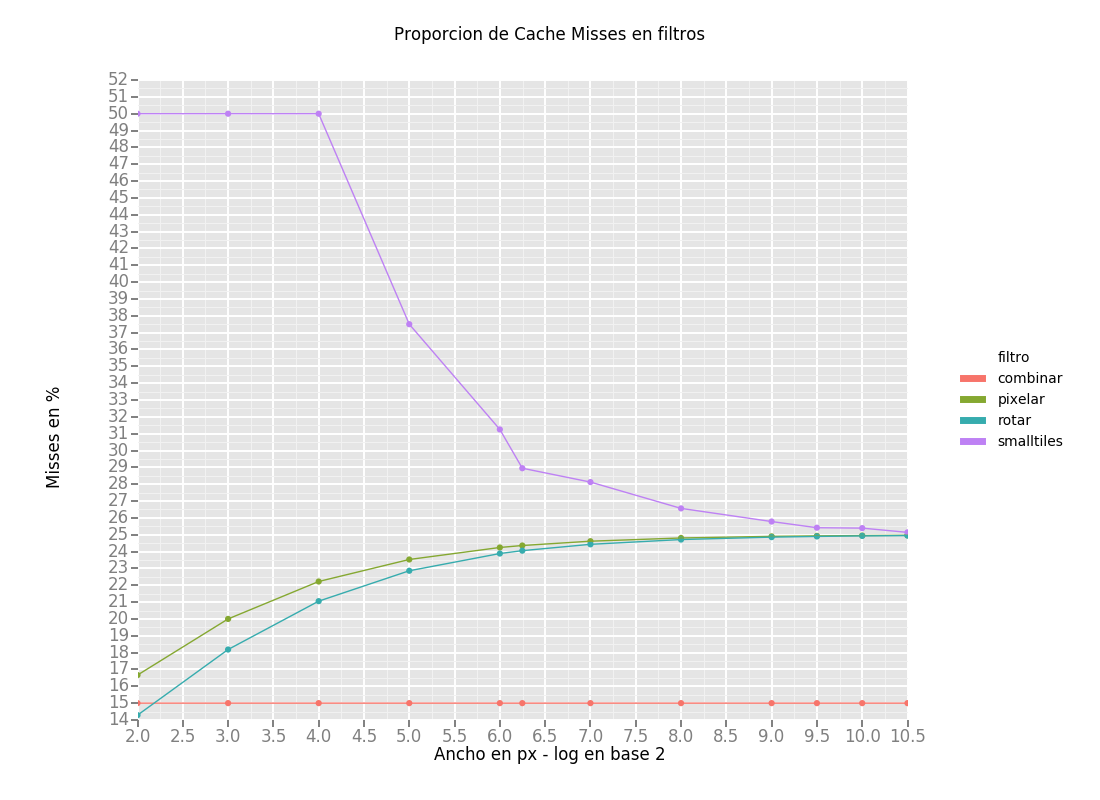
\includegraphics[scale=0.6]{imagenes/diagramas/graficos/ProporcionCacheMissesEnFiltros.png}
	\caption{Comparación de misses entre filtros}
	\label{ProporcionCacheMissesEnFiltros}
  \end{center}
\end{figure}

Analisis de tiempos, combinar es esperable porque tiene mas procesamiento y floats. Puntos interesantes, pixelar y rotar es casi un espejo invertido comparado con el cache. Smalltiles tiene comportamientos particulares en algunos puntos.

\begin{figure}[!htb]
  \begin{center}
	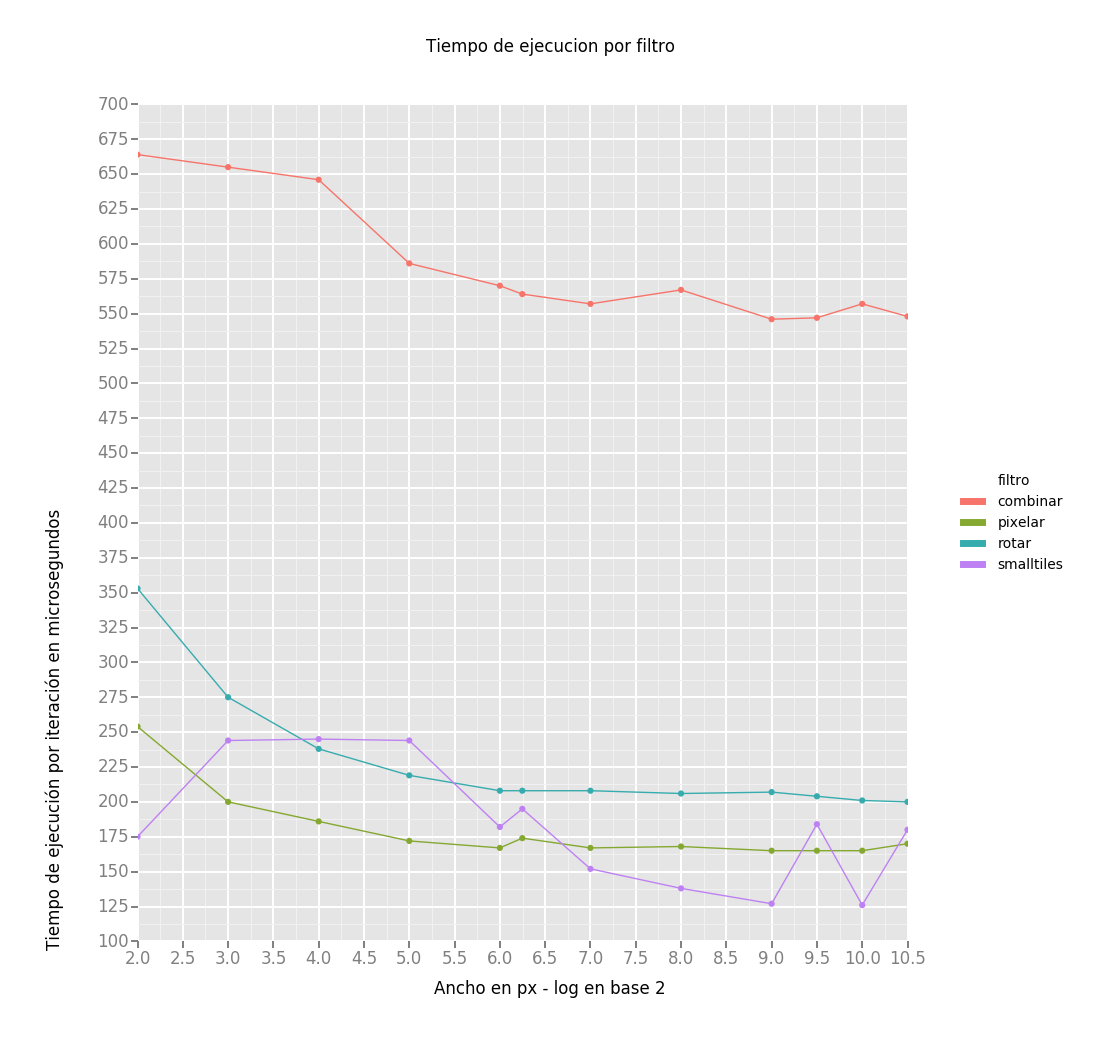
\includegraphics[scale=0.6]{imagenes/diagramas/graficos/TiemposDeEjecucionEnFiltros.png}
	\caption{Tiempo de ejecucion entre filtros}
	\label{TiemposDeEjecucionEnFiltros}
  \end{center}
\end{figure}

\subsubsection*{Comportamiento en anchos muy pequeños}

Cambiar subtitulo. Uso pixelar porque hace lecturas a la linea superior de cada px procesado, por ende podemos jugar con el ancho de la imagen comparando con el ancho de la linea de cache.

Analizar la proporcion de misses con respecto a la cantidad de instrucciones por iteracion y compararlo con la relacion entre las instrucciones y cuanto duro cada iteracion.

Los graficos encajan bastante en cuanto a misses y cuantas instrucciones lee

Se puede analizar el porque hay menos misses en imagenes con 7px, 11px, 15px, etc. comparadas con los multiplos de 4 (8, 12, 16 etc)

\begin{figure}[!htb]
  \begin{center}
	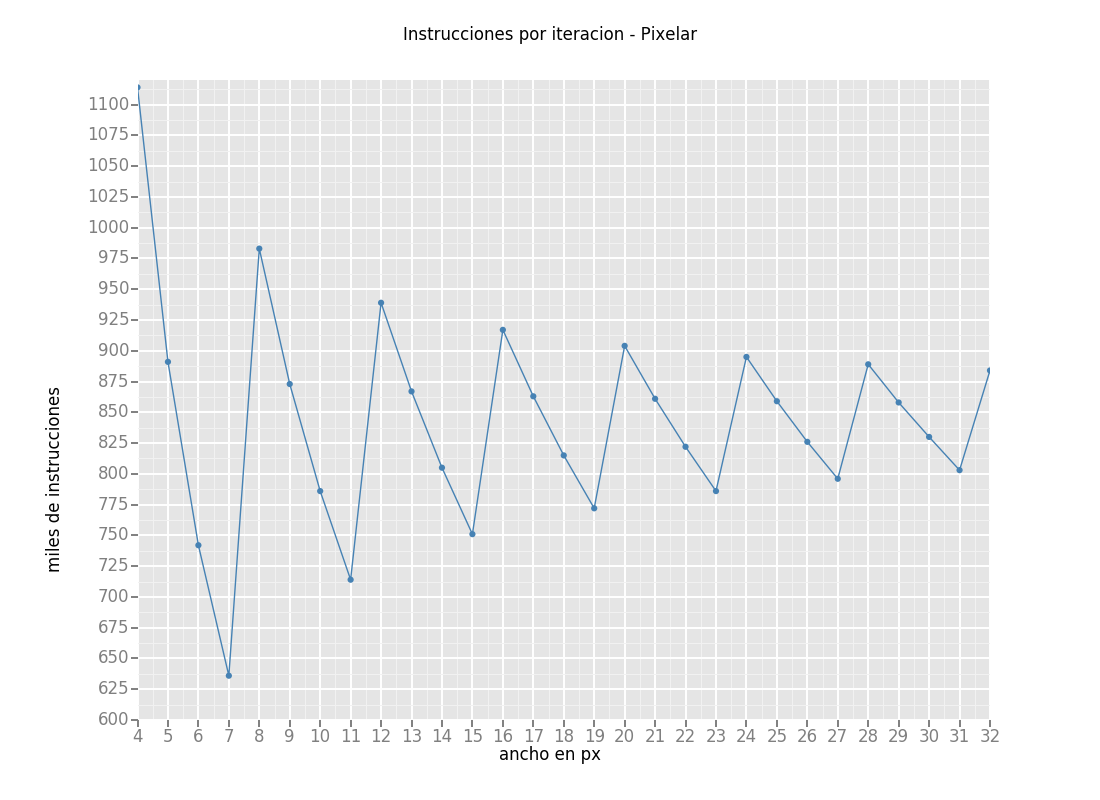
\includegraphics[scale=0.6]{imagenes/diagramas/graficos/LowWidthInstruccionesPixelar.png}
	\caption{Tiempo de ejecucion entre filtros}
	\label{LowWidthInstruccionesPixelar}
  \end{center}
\end{figure}

\begin{figure}[!htb]
  \begin{center}
	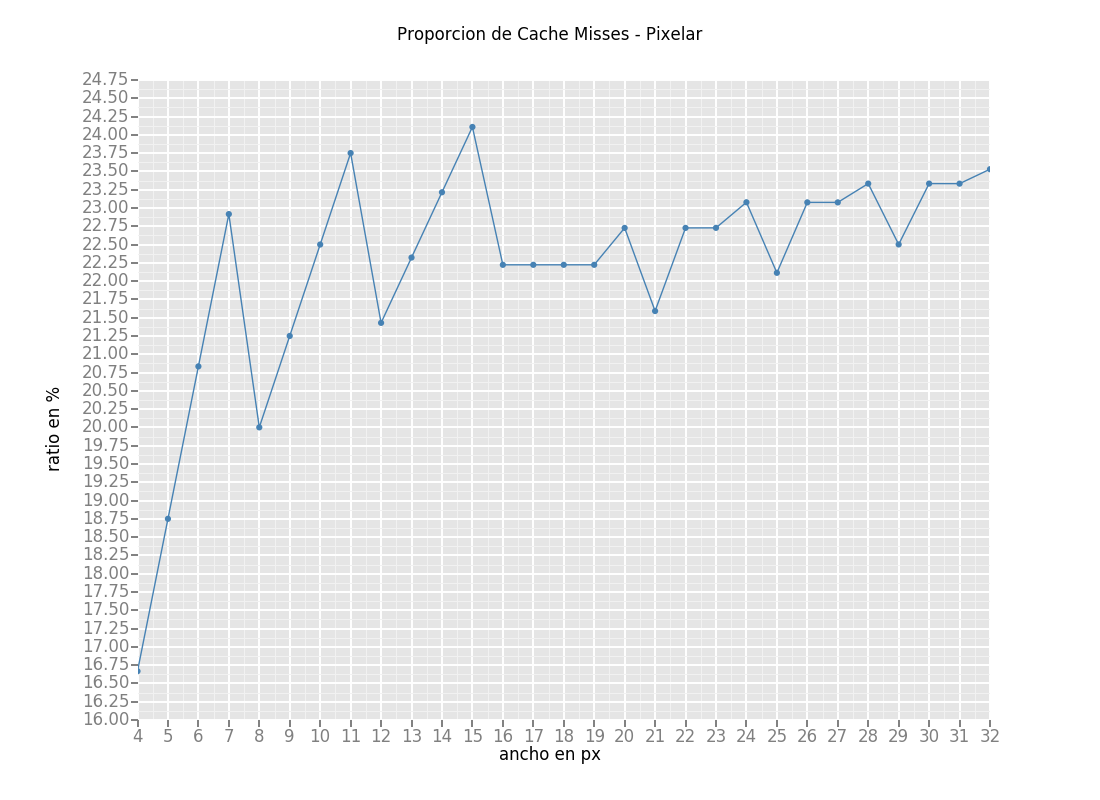
\includegraphics[scale=0.6]{imagenes/diagramas/graficos/LowWidthCacheMissesPixelar.png}
	\caption{Tiempo de ejecucion entre filtros}
	\label{LowWidthCacheMissesPixelar}
  \end{center}
\end{figure}

\begin{figure}[!htb]
  \begin{center}
	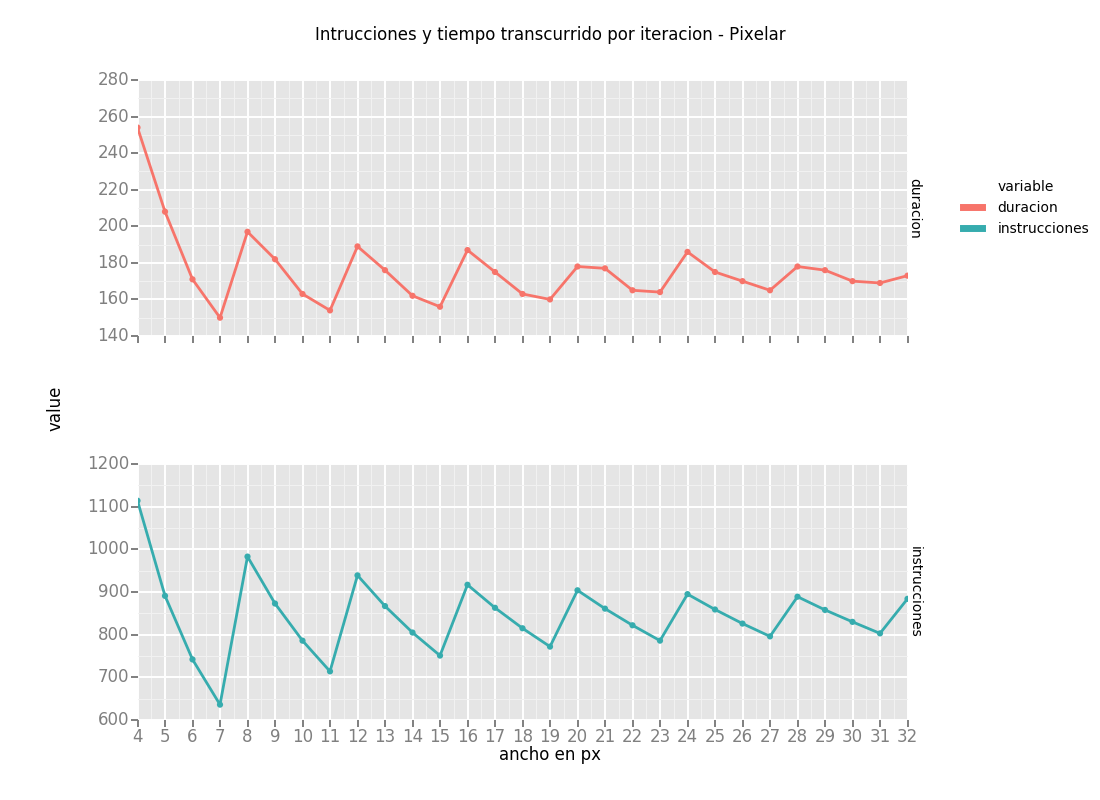
\includegraphics[scale=0.6]{imagenes/diagramas/graficos/LowWidthCacheMissesEInstruccionesPixelar.png}
	\caption{Tiempo de ejecucion entre filtros}
	\label{LowWidthCacheMissesEInstruccionesPixelar}
  \end{center}
\end{figure}

\section{Conclusiones y trabajo futuro}





\end{document}


